%%%%%%%%%%%%%%%%%%%%%%%%%%%%%%%%%%% CABECALHO %%%%%%%%%%%%%%%%%%%%%%%%%%%%%%%%%%%
\documentclass[a4paper]{abntex2}

\usepackage[utf8]{inputenc}
\usepackage{csquotes}
\usepackage[brazil]{babel}
\usepackage[T1]{fontenc}
\usepackage{pifont}
\usepackage{xcolor,graphicx}
\usepackage{sidecap}
\usepackage[all,defaultlines=2]{nowidow}
\usepackage[multiple]{footmisc}
\usepackage{enumitem}
\usepackage{fmtcount}
\usepackage{multirow}
\usepackage[backend=bibtex,backref=true]{biblatex}
\bibliography{projeto.bib}
\hypersetup{
	colorlinks=true,
	urlcolor=blue,
	linkcolor=black,
	citecolor=red
}


\author{Igor~Santos\\
	Universidade Estácio de Sá\\
	Rio de Janeiro, RJ\\
	\texttt{igorsantos07+conf@gmail.com}
}
\title{Projeto~de~TCC\\TheConf}

\makeindex
\begin{document}
\pagenumbering{gobble}
\maketitle

%%%%%%%%%%%%%%%%%%%%%%%%%%%%%%%%%%%%%%%% INICIO %%%%%%%%%%%%%%%%%%%%%%%%%%%%%%%%%%%%%%%%

\chapter*{Prefácio}
\section*{Definições usadas neste documento}
Para fins de comunicação, as seguintes palavras são tidas como sinônimo, exceto quando especificado o contrário -- na seção \ref{sec:eventos} explicaremos os conceitos envolvidos mais a fundo:
\begin{itemize}
	\item Conferência
	\item Congresso
	\item Evento
\end{itemize}
\newpage

\pagenumbering{arabic}
\tableofcontents

\chapter{Proposta do Projeto de TCC}

%%%%%%%%%%%%%%%%%%%%%%%%%%%%%%%%%%%%%%%%%%%%%%%%%%%%%%%%%%%%%%%%%%%%%%%%%%%%%%%%%%%%%%%%%
\section{O Projeto}

É notável a dificuldade que conferencistas possuem, muitas das vezes, em obter informações atualizadas sobre as conferências das quais participarão ou estão participando naquele momento. Esta opinião foi compartilhada por diversas pessoas informalmente consultadas.

Por exemplo, muitas vezes são entregues panfletos ou cartões com a programação, mas esse tipo de objeto frequentemente se perde ou se danifica no decorrer do dia. Sem contar as possíveis alterações de última hora, o que torna a grade distribuída alvo de rabiscos e anotações. Invariavelmente, \emph{slots} de programação indefinida (comum em mesas-redondas ou \emph{lightning talks}\footnotemark) levam o conferencista a se deslocar até o lugar para descobrir se valerá a pena assistir ou não -- ou simplesmente não atender ao \emph{slot}.

Partindo destas premissas, o objetivo do Projeto é criar um aplicativo móvel que permita aos usuários obterem as diversas informações referentes ao evento do qual participam, em tempo real. Informações como: a liberação da grade de programação, atualizações e mudanças da mesma; dados de contato dos palestrantes; detalhes sobre o processo e valores das inscrições; localização e como chegar ao local; comércio e atrações da região; notícias e novidades sobre a conferência em geral. Este aplicativo teria um backend facilmente acessível, onde os organizadores poderiam inserir tais informações.

\footnotetext{Série de palestras de curta duração, dadas pelos próprios conferencistas}

%%%%%%%%%%%%%%%%%%%%%%%%%%%%%%%%%%%%%%%%%%%%%%%%%%%%%%%%%%%%%%%%%%%%%%%%%%%%%%%%%%%%%%%%%
\subsection*{Opções de nome}

Seguem aqui alguns componentes que podem ser utilizados de inspiração, e algumas sugestões já pensadas para o nome do sistema:\\

\begin{tabular}{rl|c|c}
\multicolumn{2}{c|}{\textbf{Afixos}} & \textbf{Substantivos} & \textbf{Sugestões} \\\hline
Bit		& Data	& Congresso		& \multirow{6}{6cm}{EvenTime \footnotemark, BitConf, Dataconf, QuickConf, ClickConf, HandyConf, The Event, The Conf} \\\cline{1-3}
Time	& App	& Conferência	& \\\cline{1-3}
Quick	& Fast	& Conf			& \\\cline{1-3}
Rápido	& Veloz	& Evento		& \\\cline{1-3}
Click	& Lite	& Event			& \\\cline{1-3}
Handy	& The	& 				& \\
\end{tabular}
\footnotetext{EvenTime pode soar como \emph{Even+Time}}


%%%%%%%%%%%%%%%%%%%%%%%%%%%%%%%%%%%%%%%%%%%%%%%%%%%%%%%%%%%%%%%%%%%%%%%%%%%%%%%%%%%%%%%%%
\section{Método de Trabalho}
O objetivo principal deste projeto é produzir um sistema de mercado, confiável e que possa ser usado por congressistas e organizadores de eventos para melhoria da comunicação. Para que tenhamos sucesso, é essencial ter um procedimento sólido para o entendimento do projeto e do que deve ser feito, e uma metodologia eficiente de desenvolvimento.

\subsection{Metodologia de análise e avaliação das premissas do projeto}
Para tanto, considerando o fator inovador da ideia, foi decidido adotar a metodologia da Startup Enxuta, ou \emph{Lean Startup} como é mais conhecida. O conceito principal por trás dela é o \emph{Customer Discovery}\cite{manual-startup}, cujo objetivo é pesquisar o mercado e identificar suas características. Esse processo consiste de pesquisas e análises de mercado, enquetes e entrevistas com possíveis clientes, a fim de avaliar a viabilidade do projeto e comparar as hipóteses iniciais com os anseios e problemas reais dos clientes.

A principal vantagem do \emph{Customer Discovery} é a tranquilidade de construir uma empresa baseada em fatos reais e sólidos, ao invés de trabalhar em cima de premissas incertas e que podem ser falhas. É essencial saber em que terreno estamos pisando, de forma a gerar o máximo de valor para o cliente, e assim obter feedback sincero sobre o progresso do sistema. A partir desse feedback é possível re-desenhar o projeto, de forma a atingir as expectativas dos usuários e obter melhor aceitação no mercado.

\subsection{Metodologia de desenvolvimento}
Seguindo as ideias do Movimento Agile, que em parte também inspiraram a \emph{Lean Startup}, o desenvolvimento do projeto consistirá principalmente de diversas iterações curtas entre criação, testes e apresentação aos usuários, para que o feedback seja recebido rapidamente e inserido no próximo ciclo de iterações.

Para organizar o desenvolvimento, as tarefas serão geridas a partir da área de \emph{Issues} do \emph{BitBucket}. Lá é possível criar tarefas, categorizar e priorizar, delegar e ordenar. O andamento do projeto será acompanhado a partir de \emph{milestones} configurados na mesma área, todos com claras datas de finalização.

O \emph{BitBucket}, além de possuir um subsistema de tarefas, serve principalmente para armazenar na \emph{cloud} um servidor centralizado de \emph{git}. Desta forma temos também um sistema eficiente de backup de código. Ele também participa do ambiente da companhia, auxiliando a entender o histórico de desenvolvimento no decorrer do tempo. Sistemas de versionamento como o \emph{git} armazenam todas as alterações de código que foram feitas, nos ajudando a analisar a produtividade e encontrar, de forma simples, os responsáveis por determinadas partes do sistema.

Por fim, para organizar o fluxo de código, será utilizado o \emph{GitFlow}\cite{gitflow} uma metodologia de versionamento que organiza as \emph{tags} de um repositório de forma clara e lógica. A organização eficaz desse sistema nos permite criar um ciclo contínuo de \emph{deploys}, e futuramente implementar um sistema de Integração Contínua\footnotemark{} que irá se adaptar facilmente ao gerenciamento que já teremos.

\footnotetext{Integração contínua é o nome de um ciclo ininterrupto de desenvolvimento que visa a entrega fixa de pequenos pacotes. Novas funcionalidades ou correções e alterações são sempre acompanhadas de testes automatizados, que, quando tem resultado positivo, possibilitam a atualização do sistema em produção ou outras tarefas cotidianas do projeto, tudo de forma automatizada.}

\begin{figure}[!hb]
	\centering
	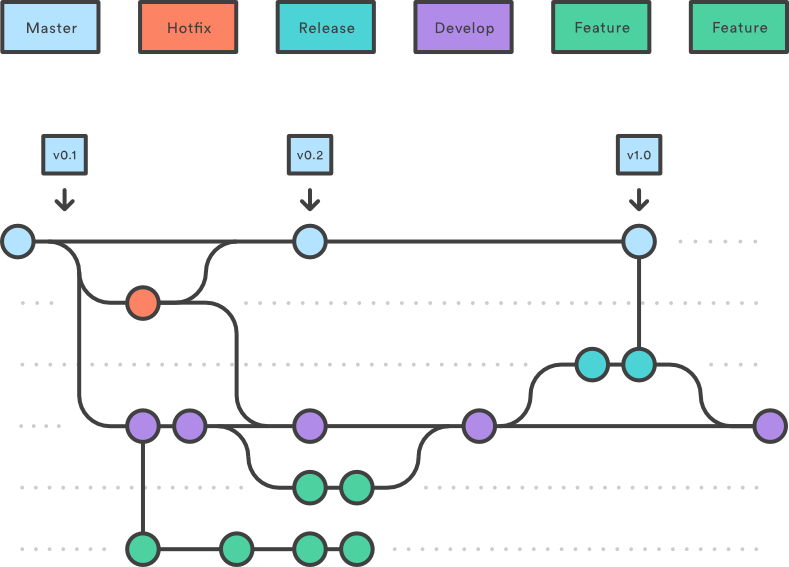
\includegraphics[width=0.7\linewidth]{imagens/gitflow.png}
	\caption{Exemplo de como \emph{GitFlow} funciona, exibindo os diversos \emph{branches} da metodologia.}
\end{figure}


%%%%%%%%%%%%%%%%%%%%%%%%%%%%%%%%%%%%%%%%%%%%%%%%%%%%%%%%%%%%%%%%%%%%%%%%%%%%%%%%%%%%%%%%%
\chapter{A Empresa e o Negócio}
% Aqui precisamos falar sobre o historico e atividade da empresa (aka quem é o cara por trás da empresa, já que ela ainda não existe), o mercado, a concorrencia e escalabilidade do negocio. Boa parte disso aparece no BMC mas nem tudo, então tem que ficar de olho

%%%%%%%%%%%%%%%%%%%%%%%%%%%%%%%%%%%%%%%%%%%%%%%%%%%%%%%%%%%%%%%%%%%%%%%%%%%%%%%%%%%%%%%%%
\section{Histórico}

%%%%%%%%%%%%%%%%%%%%%%%%%%%%%%%%%%%%%%%%%%%%%%%%%%%%%%%%%%%%%%%%%%%%%%%%%%%%%%%%%%%%%%%%%
\section{\emph{Business Model Canvas} - Um Modelo de Negócios provisório}
% Explicar porque o BMC é uma boa estratégia para o projeto/empresa

% detalhar em subseções cada um dos nove pontos do BMC

% Aqui indicam que o mercado de eventos movimenta 70bi/ano no Brasil: http://revistapegn.globo.com/Revista/Common/0,,EMI330736-17180,00.html

\subsection{Os tipos de eventos científicos e tecnológicos} \label{sec:eventos} % injetar isso em algum ponto do BMC

%%%%%%%%%%%%%%%%%%%%%%%%%%%%%%%%%%%%%%%%%%%%%%%%%%%%%%%%%%%%%%%%%%%%%%%%%%%%%%%%%%%%%%%%%
\section{Concorrência}
Não foi encontrada nenhuma empresa que preste serviços diretamente relacionados ao espectro do mercado que pretendemos cobrir com nosso projeto. No entanto, há algumas empresas relacionadas à organização de eventos ou venda de ingressos que são dignas de nota. Em especial, a Sympla, EventBrite e Eventick são consideradas parcialmente concorrentes, pois há uma possibilidade de futuramente também vendermos entradas para os eventos indicados no aplicativo. Enquanto este não é nosso foco inicial, é um caminho natural a seguir no ramo, como atividade secundária.


\subsection*{Interevent}
Esta empresa foi indicada por uma usuária do ramo das Ciências Biológicas, quando consultada sobre a ideia geral deste projeto. É uma empresa carioca que, desde 2006, presta serviços completos de planejamento, organização, divulgação e administração de congressos. Aparentemente, não há nenhum serviço especificamente voltado para o público móvel, e a comunicação interna durante o evento se resume ao tradicional material impresso distribuído.

\subsection*{Sympla}
A Sympla é uma \emph{startup} mineira de venda online de ingressos e gestão de eventos, de quase 3 anos de mercado. Ela foi eleita pela revista Exame \emph{"uma das 8 startups mundiais para ficar de olho em 2015"}\cite{exame-8-startups}. Concorre no mercado nacional com empresas internacionais como Eventbrite e Eventick, mas possuindo vantagens competitivas, além do serviço localizado.

\subsection*{Eventbrite}

\subsection*{Eventick}

\subsection*{Meetup}


%%%%%%%%%%%%%%%%%%%%%%%%%%%%%%%%%%%%%%%%%%%%%%%%%%%%%%%%%%%%%%%%%%%%%%%%%%%%%%%%%%%%%%%%%
\section{Premissas e Restrições ao Projeto}
% Acredito que aqui vai ser preciso falar das pesquisas que vamos rodar pra avaliar todas as hipoteses, e quais sao elas e como as pesquisas ajudariam a valida-las. Talvez isso seja encaixável no BMC também por causa da necessidade de descrever as hipóteses e os testes sobre ele

%%%%%%%%%%%%%%%%%%%%%%%%%%%%%%%%%%%%%%%%%%%%%%%%%%%%%%%%%%%%%%%%%%%%%%%%%%%%%%%%%%%%%%%%%
\chapter{Os Sistemas Atuais}

%%%%%%%%%%%%%%%%%%%%%%%%%%%%%%%%%%%%%%%%%%%%%%%%%%%%%%%%%%%%%%%%%%%%%%%%%%%%%%%%%%%%%%%%%
\section{Principais Concorrentes}
Para o entendimento mais aprofundado do mercado atual é necessário analisar as atividades exercidas pelas empresas concorrentes. Aqui será demonstrado o que foi encontrado sobre os sistemas atuais no que tange seu funcionamento e aspectos de mercado.

\subsection{Interevent}
\subsubsection*{Tecnologia e serviços oferecidos}
A empresa possui uma solução aparentemente completa para a organização e gerenciamento de congressos. Eles cobrem áreas como:
\begin{itemize}[itemsep=-1ex]
	\item Áreas de exposição, controle, prospecção e comunicação com patrocinadores;
	\item Recebimento de inscrições e credenciamento;
	\item Envio de newsletters;
	\item Planejamento financeiro e suporte na conciliação bancária;
	\item Auxílio na criação da identidade visual do evento e contratação de assessoria de imprensa;
	\item Auxílio no planejamento do evento, como definição de local e cronograma, reuniões, indicação de fornecedores e hotéis confiáveis;
	\item Administração de palestrantes e suas reservas, passagens, etc, e organização da grade de palestras;
	\item Geração de hotsite com atualizações, inscrições e envio de trabalhos;
	\item Gerenciamento completo no decorrer do evento, com staff próprio, logística, e programação especial pré, pós-evento, e durante o mesmo para os acompanhantes dos congressistas.
\end{itemize}

\subsubsection*{Mercados atingidos}
Em sua home page\cite{interevent}, a Interevent exibem 21 eventos. Cerca de somente nove deles são do ano de 2014. A maioria esmagadora de eventos é do mercado médico, cobrindo áreas como dermatologia, neurologia, oncologia, nutrição, patologia, biologia celular, dentre outros. Dos congressos anunciados na página inicial, somente um deles fica fora: um sobre fomento comercial. Portanto, é possível notar claramente o foco da empresa no mercado de eventos de medicina. Além do ramo de organização de congressos, a Interevent também oferece serviços de gerenciamento de sociedades e planejamento de eventos corporativos privados.

\subsubsection*{Receita}
Não foram encontrados detalhes explícitos sobre a forma de receita da empresa ou seu faturamento. Estima-se que, devido ao tamanho dos congressos organizados, a baixa quantidade de eventos anualmente, e o grande espectro de assessorias oferecidas, a companhia tenha seu rendimento baseado em altas somas cobradas das entidades organizadoras pelos serviços.

\subsubsection*{Vantagens e Desvantagens no mercado}
Analisando o material disponível publicamente e a entrevista com a usuária citada, foram identificadas as seguintes deficiências:
\begin{itemize}
	\item Muitas atividades ainda são manuais, como por exemplo a homepage de divulgação dos eventos -- há links para hotsites com erro no endereço (exemplo: \emph{interevent.\underline{com..br}/evento/sbdof2015}) --, certificados com nomes distintos dos usados na inscrição, dentre outros;
	\item Os hotsites dos congressos é de difícil acesso, pois depende de parâmetros na URL que são variáveis e difíceis de gravar. A usuária citou ser frustrante (e constante) ir no Google para precisar buscar o site do evento, e acidentalmente clicar no site oficial da associação ou sociedade, ao invés da página desejada. Isso poderia ser facilmente resolvido com uma URL amigável, indicando o ano/nome do evento no subdomínio ou \emph{path};
	\item Foram encontrados diversos problemas de desenvolvimento em produção, como: erros de \emph{JavaScript} que impossibilitam a interface de funcionar corretamente; uma página em branco, somente com uma mensagem de erro de \emph{query} do \emph{MySQL}; além da reclamação por parte da usuária sobre encontrar dificuldades técnicas diversas vezes ao acessar a página de emissão de certificado.
\end{itemize}

Há a necessidade de entrevistar outros usuários e/ou organizadores de eventos clientes da Interevent a fim de coletar feedbacks positivos e de outros pontos de vista. No entanto, inicialmente a empresa é tida como concorrência distante visto que não objetivamos atuar na mesma área, e nas áreas em que poderíamos concorrer diretamente ela possui deficiências técnicas graves - como o hotsite, por exemplo.

\subsection{Meetup}
% TODO


\section{Outros Concorrentes - Venda de ingressos}
Há inúmeras empresas no mercado de venda de ingressos por sistemas digitais. Aqui estaremos descrevendo as maiores, e sumarizando as principais características de todas. As empresas discutidas aqui são voltadas para o mercado de eventos de pequeno e médio porte, principalmente. Para eventos maiores, empresas como a TicketMaster e Ingresso.com dominam o mercado (internacional e nacional, respectivamente). As companhias citadas abaixo surgiram para preencher a lacuna dos eventos menores, e aqueles de maior porte estão muito fora do escopo do nosso projeto.

\subsection{Sympla}

\subsubsection*{Tecnologia e serviços oferecidos}
O site é moderno e parecem antenados com as novidades do mercado, implementando tecnologias atuais e facilitando todo o processo de venda de ingressos e credenciamento de participantes. Eles dão suporte a diversos tipos de eventos, mas o mercado principal que conseguiram -- ou desejaram -- atingir foi o de eventos de entretenimento, como festas, shows, etc. No entanto, a empresa oferece suporte a um grande espectro de eventos, como congressos e seminários, cursos e workshops, eventos religiosos, corporativos, esportivos, gastronômicos e de entretenimento, encontros e networking, e eventos online também. Alguns dos recursos oferecidos pela Sympla a seus clientes são\cite{sympla-features}:
\begin{itemize}[itemsep=-1ex]
	\item Divisão de tarefas de gerenciamento com diversos usuários, com níveis de acesso;
	\item Organização de uma rede de promoters;
	\item E-mail marketing para o público de eventos passados;
	\item Fechamento financeiro de todos os canais de venda;
	\item Certificados de participação;
	\item Acompanhamento de origem do público via \emph{Google Analytics};
	\item Checkin facilitado com um aplicativo, que lê QR-Codes no ingresso;
	\item Tecnologia de impressão de ingressos moderna e anti-fraude;
	\item Venda de ingressos com organização de lotes e página personalizável;
	\item Também há um pacote especial de serviços que inclui staff de suporte aos clientes durante a venda, credenciamento no evento e destaque na divulgação nos canais da Sympla.
\end{itemize}

\subsubsection*{Mercados atingidos}
A Sympla indica que já realizou mais de 14 mil eventos em mais de 1.700 cidades, e já atingiu mais de 4 mil produtores. Há uma série de casos de sucesso publicados\cite{sympla-cases}, apesar de alguns ramos ainda não terem sido citados -- como eventos religiosos ou congressos e seminários (os dois últimos sendo uns de nossos principais focos):
\begin{itemize}[itemsep=-1ex]
	\item Diversos na área de entretenimento;
	\item Eventos esportivos -- \emph{Quanta Sports} com corridas de rua, e \emph{Trilogy Sports} com esportes de aventura;
	\item Cursos/workshops -- \emph{Vila de Produções};
	\item Seminários -- \emph{TED}\footnotemark, no \emph{TEDxBH} (outro dos nossos focos);
	\item Corporativos e de nicho -- como no mercado pecuário.
\end{itemize}
\footnotetext{Evento de palestras curtas e inovadoras, sobre tópicos diversos. Bem famoso e possui versões mundo afora.}

\subsubsection*{Receita}
O método de receita da startup é baseado na porcentagem de 10\% do que for vendido em ingressos -- valor também usado para pagar taxas administrativas de cartões de crédito. Eventos gratuitos não são cobrados. A receita restante dos ingressos é repassada aos produtores em tempo real, através de pequenos depósitos, ou de uma vez só, no terceiro dia útil após o término do evento. Não há informação sobre vantagens e desvantagens dos dois métodos de recebimento.

\subsubsection*{Vantagens e Desvantagens no mercado}
A Sympla é uma empresa moderna e que está sendo acelerada na região de BH, um dos berços de startups do Brasil. Recebeu, segundo estimativas, ao menos dois aportes de fundos de investimento e investidores individuais, sendo o segundo de cerca de R\$ 2 milhões.\cite{sympla-aporte}

Seu ponto forte é a modernidade dos sistemas e a simplicidade dos serviços que oferecem, que facilitam a vida do produtor, o tirando do trabalho de conferência de público, venda de ingressos -- e verificação de autenticidade --, dentre outras burocracias da área.

No entanto, há pouco foco em distinção entre os tipos de eventos cobertos, oferecendo praticamente o mesmo pacote de serviços a todos eles. Eventos mais elaborados e específicos, como os do mercado técnico-científico podem ficar em desvantagem com um produto focado somente na venda dos ingressos e, parcialmente, na gestão financeira e na divulgação -- quando há muito mais por trás desse mercado. Neste ponto, a Interevent tem uma vantagem clara, pois oferece pacotes de serviços que cobrem todas as tarefas de organização de congressos, de uma ponta a outra.

\subsection{Eventbrite}
A empresa que iniciou o mercado de venda de ingressos digitais. Foi fundada ainda em 2006 em São Francisco, e atualmente emprega mais de 500 funcionários ao redor do mundo. A empresa já recebeu mais de \$140 milhões em investimentos públicos entre 2011 e 2013, sem contar os investimentos iniciais não divulgados por companhias como Sequoia Capital, DAG Ventures e Tenaya Capital. \cite{eventbrite-wiki}

\subsubsection*{Tecnologia e serviços oferecidos}
A empresa possui como objetivo cobrir todos os aspectos do processo de vendas e credenciamento de participantes de um evento. Se por um lado, eles se focam somente nisso, por outro eles o fazem muito bem, sendo referência no mercado nesse sentido. Para tanto, eles oferecem a seguinte gama de serviços e funcionalidades:
\begin{itemize}
	\item Venda de ingressos com diferentes tipos de entradas, e com a possibilidade de distribuição de cupons de desconto também;
	\item Página inicial e aplicativo com listagem atrativa dos eventos locais, e categorias principais - artes, gastronomia, música, cursos, networking e festas;
	\item O evento tem sua página de conteúdo personalizada, com mapa de localização, detalhes e informações de contato da organização -- mas o foco principal é o box de venda de ingressos;
	\item Integração com mídias sociais, permitindo o compartilhamento do evento após a compra -- segundo suas pesquisas, isso aumenta consideravelmente o alcance do evento;
	\item Possibilidade de coletar dados diversos dos participantes, como título, site, ou campos personalizados -- útil para preenchimento de identificações de conferências;
	\item Relatórios robustos sobre os participantes, como dados de contato, informações gerais e engajamento, e informações financeiras do evento;
	\item Suporte 24h por dia, 7 dias por semana para os organizadores e participantes;
	\item Plataforma Neon: venda de ingressos no local do evento com impressora de mercado (conhecida como \emph{BOCA}), e credenciamento a partir de aplicativo próprio, com pessoal próprio também;
	\item Sistema de coleta de doações para eventos políticos ou de arrecadação de fundos.
\end{itemize}

\subsubsection*{Mercados atingidos}
O principal público-alvo da Eventbrite é o mercado de eventos de entretenimento de pequeno e médio porte. Recentemente eles têm tentado entrar no mercado de grande porte também, mas ainda reconhecem de forma clara que esta área pertence a empresas tradicionais como a Ticketmaster: ``Se o topo da pirâmide é Lady Gaga no Madison Square Garden, com certeza esse território é da Ticketmaster. Mas absolutamente todo o restante é da Eventbrite.'' -- tradução livre de fala de Julia Hartz, co-fundadora e presidente da Eventbrite, em matéria da Forbes\cite{eventbrite-lucro-forbes}. Apesar disso, eles já cobrem grandes festivais, como o Governor's Ball de Nova Iorque de 2013.\cite{eventbrite-lucro-forbes}

O foco principal de eventos deles são os de entretenimento em geral, como shows, apresentações musicais, teatrais e culturais em geral, e secundariamente inscrições para cursos e workshops avulsos, encontros de palestras, e etc. Também possuem apelo no mercado esportivo e outros menores. No entanto, eles não possuem nenhum chamariz específico para nenhuma destas áreas, sendo um sistema essencialmente genérico e focado na divulgação dos eventos e venda dos ingressos, funcionando de forma simplificada e fluida para os organizadores e participantes. O principal diferencial entre eles e seus grandes concorrentes é a simplicidade de criar um evento: não há necessidade de contato com agente de vendas, detalhes de cartão de crédito ou as burocracias comuns do meio; o cadastro do evento é feito de forma similar ao cadastro de um novo usuário num sistema comum.

\subsubsection*{Receita}
De acordo com o relatório anual de 2013 da empresa, foram vendidos 58 milhões de tickets, totalizando \$960 milhões, o que totaliza um mínimo de \$24 milhões em lucro de vendas, considerando a taxa de 2,5\% por ingresso vendido. Como a companhia não cobra por eventos gratuitos, não há como estimar a renda proveniente da taxa fixa de \$0,99 por ingresso já que não há divulgação da porcentagem desse tipo de evento no portfólio.\cite{eventbrite-lucro-tnw}. A empresa foi citada na Forbes com declarações altamente positivas sobre seu estado financeiro e futuro da empresa.\cite{eventbrite-lucro-forbes}.

\subsubsection*{Vantagens e Desvantagens no mercado}
No caso da Eventbrite, não há nenhuma distinção nos serviços fornecidos para diferentes tipos de eventos. É notável, por exemplo, a deficiência do sistema com relação a eventos como conferências, onde informações sobre alimentação, interesse em workshops, passagens aéreas e afins também se fazem necessárias\cite{eventbrite-review}. No entanto, é possível buscar no site por categorias diversas -- como cursos, conferências, esportes, gastronomia, música, eventos sem fins lucrativos e de arrecadação de fundos, artes performáticas e até eventos políticos.

Outra desvantagem é que as páginas dos eventos focam essencialmente na venda, contendo informações sobre a programação mas de forma secundária -- o que força os organizadores a manter seus próprios hotsites, quando o evento não é simples demais. Aliás, não há integração transparente: sempre haverá o logotipo laranja e chamativo da Eventbrite em algum lugar das páginas sob controle deles, os ingressos, e no uniforme dos \emph{staffs} no dia do evento.

Por fim, outro ponto menos relevante a ressaltar é que, para eventos de grande porte, as taxas cobradas passam a ficar um pouco salgadas, pois como o valor pago é proporcional ao valor do ingresso, quanto mais cara a entrada é, mais será pago.

A maior vantagem é sua inserção no mercado internacional: a empresa é a líder do mercado americano, e despertou diversos clones mundo afora -- só nos EUA parecem ter mais de 170 clones, tanto genéricos como de nicho\cite{eventbrite-concorrencia}; alguns possuem funcionalidades ou precificação um pouco diferenciada\cite{eventbrite-concorrencia-quora}, mas ainda são considerados clones. Eles não possuem versão nacional ainda, mas se encarregaram de entrar no mercado latino-americano comprando uma startup-clone: a Eventioz -- que também atende Argentina, Chile, Colômbia, México e Peru. Para os outros 13 países atendidos há versões com domínios locais e traduzidas, quando necessário.

\subsection{Eventioz - uma empresa Eventbrite}
A Eventioz é uma startup clone da Eventbrite que nasceu na Argentina em 2008. Até 2011 eles já estavam operando no México, Chile, Colômbia e Peru, e chegaram ao Brasil em 2013. No final do mesmo ano, foram comprados pela Eventbrite, como forma desta empresa se expandir para o mercado latino.

\emph{\textbf{Nota:} não confundir com a Eventials, empresa brasileira de transmissão de webinars.}

Seu funcionamento e recursos são bem similares ao já oferecido pela Eventbrite -- a principal diferença sendo o fato de terem suporte local na América Latina, e versões localizadas do sistema (no entanto, o português em alguns pontos parece mal-traduzido do espanhol). No entanto, não é ainda o mesmo sistema, o que significa que a interface para um usuário do Eventbrite será diferente, e a lista de funcionalidades também pode mudar. Seguem aqui as principais diferenças:
\begin{itemize}[itemsep=-0.5ex]
	\item[(+)] parece permitir a criação de uma página mais elaborada do evento, com imagens, notícias dos palestrantes, agenda, e integração mais profunda com redes sociais;
	\item[(+)] criação automática de modelos de crachás, prontos para serem impressos;
	\item[(+)] possibilidade de inscrições de equipes ou venda de ingressos em grupo, e distribuição de termo de responsabilidade (para eventos esportivos, neste caso);
	\item[(-)] a página da empresa tem menos conteúdo, e dá destaque muito menor à busca de eventos na home;
	\item[(-)] não oferecem serviço de pessoal próprio no local do evento, ou venda na hora;
	\item[(-)] a comissão é bem mais cara: ao invés dos 2,5\% + \$0,99, são cobrados 8\% e, no caso de ingressos inferiores a R\$50, a taxa é fixa de R\$4 por ingresso vendido.
\end{itemize}

\subsection{Eventick}
A Eventick é uma startup-clone de Pernambuco, que tenta replicar o sucesso americano em território nacional, trazendo o que empresas como a Eventbrite fizeram para os moldes do Brasil. A empresa foi iniciada em 2011, e o produto foi a público em 2012.\cite{eventick-startupi} Até o momento já venderam mais de 355 mil ingressos\cite{eventick-home}, e seu foco parece ser eventos musicais e entretenimento em geral.

Em questão de funcionalidades a Eventick é muito similar aos concorrentes, mas mais simples -- vale lembrar que é uma startup em crescimento, e que provavelmente virão com novidades no futuro. Atualmente estas são as principais diferenças para o mercado atual:
\begin{itemize}[itemsep=-0.5ex]
	\item[(+)] há a opção de criar um evento secreto: provavelmente ele só seria acessível a partir de um convite direto ou com a URL;
	\item[(+)] ofertas típicas para o mercado brasileiro: opções de parcelamento do ingresso (e o recebimento não seria afetado) e pagamento via boleto bancário;
	\item[(+)] a comissão varia de cerca de 10\% a até 5\%, e depois fica fixa em R\$20 para a empresa e mais 5\% para cobrir os custos de pagamento. Isso mantém os valores cobrados mais justos tanto para eventos pequenos quanto para eventos de grande porte e com entrada mais elevada;
	\item[(-)] não há categorização ou distinção dos tipos de eventos que pretendem cobrir. O foco da empresa é em eventos de entretenimento;
	\item[(-)] não há canal de divulgação direta na home do Eventick, mas há uma página simples de busca;
	\item[(-)] também não há foco em coleta de dados dos clientes, pesquisas pós-evento, relatórios de público ou financeiro;
	\item[(-)] não parecem oferecer serviço de impressão profissional de ingressos ou aplicativo para credenciamento -- e portanto, não oferecem pessoal especializado para venda ou atendimento no evento, mas possuem serviço exclusivo de suporte aos participantes antes da ocasião.
\end{itemize}

\subsection{Show de Ingresso / SDI}
\label{sec:show-de-ingresso}
A Show de Ingressos é uma empresa com oito anos no mercado de eventos, mas com um funcionamento um pouco diferente do restante. Apesar de ser ``só mais uma'' que também vende ingressos online, eles não possuem uma plataforma tradicional onde o cliente cadastra um evento, e outras pessoas vêm comprar; a empresa fornece um sistema em cloud para que outras companhias façam seus próprios sistemas de venda de ingressos. Funciona de forma similar a sistemas de e-commerce terceirizados, mas nesse caso, para ingressos.

É possível ver dezenas de sites utilizando a chamada ``plataforma SDI'', mas em sistema de \emph{white label} -- o que significa que não fica aparente que o site é, na verdade, tercerizado. Elas são identificadas por serem divulgadas na home do Show de Ingresso, que lista diversos eventos em ordem cronológica. As páginas com detalhes dos eventos têm todas a mesma estrutura, e as taxas variam de 1,5\% até 10\%, dependendo do plano que for escolhido -- focado na venda de ingressos somente, na criação de site próprio, ou com suporte completo do SDI para criação de um sistema híbrido.

\subsubsection*{Tecnologia e serviços oferecidos}
As principais características oferecidas aos produtores e e integradores são:
\begin{itemize}[itemsep=-1ex]
	\item Controle de venda de lugares distintos, como mesas, cadeiras e lounges, com mapas;
	\item Venda de ingressos casados -- desconto para mais de um evento comprado de uma vez só;
	\item Códigos de desconto e ingressos privados para grupos de pessoas, com valores diferenciados;
	\item Dashboard de análise das vendas, com diversos filtros e opções;
	\item Sistema de cadastro de promotores e vendedores externos, cada um com URLs específicas e com controle das vendas deles de forma individualizada;
	\item Sistema de CRM, com contato com os clientes via e-mail e/ou SMS;
	\item Aplicativo de celular para facilitar o credenciamento, e o voucher pode ser digital.
\end{itemize}

Pela natureza do sistema, é possível que novas empresas sejam criadas revendendo os serviços oferecidos pela Show de Ingresso. Esse é o caso, por exemplo, da Doity: eles possuem um site igual à do Show de Ingresso, mas com um feature set reduzido e sistema de taxas diferenciado. Nesse caso, a Doity também foca em eventos técnicos, disponibilizando etiquetas de crachá, listas de credenciamento e certificados de participação.

\subsubsection*{Mercados atingidos}
O foco da empresa é em produtoras e grupos com múltiplos eventos, que vão contratar a plataforma para otimizar seus processos de vendas e enxugar os custos com TI. Outras empresas também se beneficiam do sistema, como agências de turismo e até mesmo um jornal regional online. Também há o caso de revenda do sistema, como é o caso da \emph{Doity}, citada acima.

É possível notar que, apesar de ser mais antiga no mercado, a maioria esmagadora de seus clientes se concentram na região Nordeste (Pernambuco e Bahia), apesar de haver alguns eventos no Sul-Sudeste.

\subsection{Ingresse.com}
Com cerca de dois anos de idade, a Ingresse.com é outra empresa de venda de ingressos para eventos de entretenimento. Seu foco inicial é o nicho de eventos universitários de pequeno e médio porte, mas atualmente cobre entretenimento em geral, como festas, baladas, shows, festivais e atrações culturais.

A empresa foi criada por um estudante de Manaus (da área de Economia/Psicologia), que teve a ideia durante um intercâmbio em Standford, nos EUA. Com o apoio recebido de um professor, ele abandonou o curso e voltou ao Brasil com a ideia. Formou uma equipe na sua cidade-natal, e iniciou validações do negócio em meados de 2012. Ter aberto a empresa no Amazonas foi uma vantagem, visto que é um mercado grande mas geograficamente isolado dos outros, permitindo liberdade mas sem medo de concorrência por mídia antecipada. Após encontrar o modelo de negócios mais acertado, eles se mudaram para São Paulo, onde a empresa foi fundada no início de 2013.\cite{ingresse-hypeness}\cite{ingresse-ig}

Aparentemente, no início a ideia era dar um viés de rede social ao sistema de venda de ingressos, mas esse formato foi abandonado não está mais presente no site da empresa, além dos tradicionais recursos de compartilhamento do evento.\cite{ingresse-ig}

\subsubsection*{Tecnologia e serviços oferecidos}
As \emph{features} são similares ao restante do mercado. Por ser uma empresa nova, a tendência é oferecer menos recursos, mas eles possuem algumas opções de destaque que não são o foco de alguns concorrentes, como por exemplo:
\begin{itemize}[itemsep=-1ex]
	\item Ingressos digitais e físicos com sistemas de validação e anti-fraude avançados;
	\item Aplicativos para os clientes, com busca de eventos e compra dos ingressos, e para os organizadores agilizarem o credenciamento;
	\item Otimização das páginas dos eventos para sites de busca, e divulgação via newsletters e redes sociais;
	\item Variedade nos meios de pagamento e nos métodos de recebimento para os organizadores;
	\item API para integrar o sistema de forma transparente a uma estrutura de divulgação própria -- similar ao que é possível na Show de Ingresso (\ref{sec:show-de-ingresso}), mas com foco no organizador direto e não numa promotora de eventos;
	\item \emph{Dashboard} com análise dos dados de venda e público do evento.
\end{itemize}

\subsubsection*{Receita}
No último trimestre de 2013, o primeiro ano da empresa, foi reportado um faturamento de R\$2,3 milhões. A partir dos contatos americanos do fundador, houve um aporte inicial de R\$2,5 milhões -- sendo parte vinda um fundo americano, estimado entre 1 e 2 milhões.\cite{ingresse-hypeness}


%%%%%%%%%%%%%%%%%%%%%%%%%%%%%%%%%%%%%%%%%%%%%%%%%%%%%%%%%%%%%%%%%%%%%%%%%%%%%%%%%%%%%%%%%
\section{Outros Sistemas}

%%%%%%%%%%%%%%%%%%%%%%%%%%%%%%%%%%%%%%%%%%%%%%%%%%%%%%%%%%%%%%%%%%%%%%%%%%%%%%%%%%%%%%%%%
\section{Motivações para o Novo Sistema}
% falar sobre a vantagem de usar um aplicativo com dados offline num ambiente com wifi e 3g saturados

%%%%%%%%%%%%%%%%%%%%%%%%%%%%%%%%%%%%%%%%%%%%%%%%%%%%%%%%%%%%%%%%%%%%%%%%%%%%%%%%%%%%%%%%%
\subsection{Problemas dos Sistemas Atuais}

%%%%%%%%%%%%%%%%%%%%%%%%%%%%%%%%%%%%%%%%%%%%%%%%%%%%%%%%%%%%%%%%%%%%%%%%%%%%%%%%%%%%%%%%%
\subsection{Situação Desejada}

%%%%%%%%%%%%%%%%%%%%%%%%%%%%%%%%%%%%%%%%%%%%%%%%%%%%%%%%%%%%%%%%%%%%%%%%%%%%%%%%%%%%%%%%%
\chapter{Proposta Preliminar de Sistema}
% Aqui talvez devêssemos explicar que o sistema deve ser um aplicativo móvel com interface administrativa web, e demonstrar o porque disso. 

%%%%%%%%%%%%%%%%%%%%%%%%%%%%%%%%%%%%%%%%%%%%%%%%%%%%%%%%%%%%%%%%%%%%%%%%%%%%%%%%%%%%%%%%%
\section{Requisitos do sistema}

\subsection{Requisitos funcionais}

Segue aqui uma lista não-exaustiva das funcionalidades pensadas para o sistema. Elas não estão organizadas com algum critério específico, e nem todas serão implementadas no período deste projeto. No entanto, a lista serve como referência de consulta para as pesquisas com os potenciais usuários; auxiliará na identificação de quais \emph{features} são mais importantes, ou se alguma seria pouco relevante, por exemplo. Após esta fase, com base nos resultados, será possível aferir a prioridade de cada uma das funcionalidades.


\subsubsection*{Programação do evento}
\begin{itemize}
	\item Deve ser possível visualizar os diversos \emph{time slots}:
		\begin{itemize}
			\item Eles devem ser vistos, preferencialmente, categorizados (como keynotes e palestras, lightning talks, mesas-redondas, etc);
			\item Também pode ser interessante haver uma visualização de grade, onde o usuário possa visualizar rapidamente os conflitos de horário dos slots;
		\end{itemize}
	\item Informações detalhadas sobre os slots, como:
		\begin{itemize}
			\item descrição;
			\item tópicos de interesse;
			\item palestrante(s);
			\item subcategoria - como trilhas de palestras distintas;
			\item localização, para os casos em que o evento possua mais de um ambiente;
			\item slides, quando disponíveis.
		\end{itemize}
	\item Listar todos os palestrantes e os detalhes dos mesmos, como informações de contato, mini-currículo, fotos e qual(is) slot(s) irá participar;
	\item Algumas destas informações, como subcategoria, palestrante e tópicos, podem ser utilizados para destacar ou filtrar a lista ou grade de slots;
	\item Notificações sobre lançamento das grades ou modificações nas mesmas, lançamento de slides e vídeos das palestras, dentre outros;
\end{itemize}

\subsubsection*{Trabalhos, exposições e \emph{networking}}
\begin{itemize}
	\item Para os casos em que haja exposição de patrocinadores ou trabalhos, pode ser interessante setorizar o salão de exposições e permitir a localização daqueles pelo sistema:
		\begin{itemize}
			\item Os expositores e/ou projetos podem ser buscados por palavras-chave ou por tópicos;
			\item Eles teriam um setor ou box específico do salão, e o usuário poderia facilmente localizá-lo a partir de um mapa no aplicativo ou nas entradas da área;
		\end{itemize}
	\item Auxiliar o processo de avaliação e premiação dos trabalhos apresentados:
		\begin{enumerate}
			\item Isso pode ser feito disponibilizando tablets aos avaliadores que não possuírem smartphones, ou não desejarem/puderem instalar o aplicativo;
			\item Os avaliadores lançam as notas e comentários no aplicativo conforme vêem os trabalhos;
			\item Os comentários podem ser vistos em tempo real pelos participantes do projeto avaliado;
			\item As notas são contabilizadas também em tempo real pela organização e/ou congressistas.
		\end{enumerate}
	\item Facilitar a troca de contatos nos momentos de \emph{networking} (similar ao \emph{SocialTagg}\cite{socialtagg}):
		\begin{itemize}
			\item Exibir os dados dos congressistas presentes;
			\item Permitir que contatos sejam favoritados e recebam notas;
			\item Possivelmente, permitir o download offline da base de congressistas, a partir de bases de distribuição \emph{Bluetooth} no local do evento (tecnologia conhecida como \emph{Bluetooth Marketing}).
		\end{itemize}
\end{itemize}

\subsubsection*{Informações gerais sobre o evento}
\begin{itemize}
	\item Localização do evento:
		\begin{itemize}
			\item com facilidade para identificar o trajeto via aplicativo de mapas;
			\item com indicações textuais sobre as linhas de transporte público próximas e trajetos comuns da rodoviária e aeroporto (o que pode ser útil em caso de falta de plano de dados para visualizar o trajeto ao vivo).
		\end{itemize}
	\item Indicação de locais nos arredores para:
		\begin{itemize}
			\item alimentação: uma possibilidade é integrar com o FourSquare para recomendações de lugares realmente próximos, e talvez adicionar comentários ou preferência dos organizadores sobre as opções;
			\item pontos turísticos a visitar: similar à ideia acima;
			\item hospedagem: novamente, similar às ideias acima, mas nesse caso integrando com o TripAdvisor;
		\end{itemize}
	\item Ingressos:
	\begin{itemize}
		\item Informações a venda de ingressos e as datas de mudanças de lotes;
		\item Informações detalhadas dos possíveis tipos de ingressos disponíveis;
		\item Alertas sobre o início das vendas e a mudança de lotes -- avisar, por exemplo, quando faltarem determinados dias para a troca de lote.
	\end{itemize}
	\item Exibição de feed de notícias do evento. Os organizadores devem poder lançar notas e blocos de texto maiores, sobre os quais os usuários podem ser notificados -- útil para anunciar mudanças futuras na grade, criar material de agitação entre os congressistas ou divulgações do evento em geral. 
	\item Talvez seja possível replicar a funcionalidade gerada por QR-Codes de Rede Wi-Fi e criar um link ou botão que leve o usuário a se conectar automaticamente às redes do evento, mesmo que elas possuam senha. Isso pode ser usado, inclusive, para criar redes específicas para os usuários do sistema. Veja a Figura \ref{fig:qr-wifi} como um exemplo.
\end{itemize}

\begin{SCfigure}[2.5][hb]
	\centering
	
\includegraphics[width=0.25\linewidth]{imagens/qr-wifi}
	\protect\caption[QR-Code com dados da rede Wi-Fi]{Este QR-Code possui os dados necessários para que um aplicativo leitor possa automaticamente conectar o dispositivo à rede indicada. Neste exemplo, o formato do código se lê: "\texttt{WIFI:S:<<nome da rede>>;T:<<criptografia>>;P:<<senha>>;;}". Ele foi gerado pelo aplicativo InstaWifi\cite{instawifi}, e lido com sucesso com o BarCode Scanner\cite{barcode}, ambos para Android.}
	\label{fig:qr-wifi}
\end{SCfigure}

\subsection*{Divulgação de novos eventos}
Os usuários poderão acompanhar os perfis de sociedades e associações científicas, de modo a serem notificados em primeira mão (possivelmente por email também) sobre novos eventos que estão sendo planejados - conforme eles são cadastrados na plataforma.
Esta ideia possibilita a entrada de pequenas empresas, como aquelas que organizam ciclos de palestras periódicos -- o que, em torno, ajudaria na divulgação do aplicativo web ou móvel, nos casos em que ele seria necessário para o checkin no evento.

Também é interessante disponibilizar uma integração com os eventos do Facebook, permitindo ao cliente criar um evento lá a partir da nossa plataforma. Detalhes de local e datas seriam atualizáveis automaticamente, e outras informações podem ser gerenciadas também pelo sistema -- como descrição, imagens e até mesmo novas postagens.

\subsubsection*{Redução das burocracias comuns de eventos}
\emph{Estes tópicos são principalmente secundários, pois já existem sistemas que cumprem estes papéis, pelo menos até certo nível, ou porque não encaixam muito no ambiente móvel.}
\begin{itemize}[itemsep=-0.5ex]
	\item Distribuição de pesquisas de opinião pós-evento;
	\item Controlar o credenciamento de congressistas. Aqueles que possuírem o aplicativo podem participar de uma fila especial que consistiria da leitura de um código na tela do aparelho para identificação automática do mesmo;
	\item Disponibilização de certificados de participação aos interessados, com informações sobre os trabalhos apresentados, por exemplo;
	\item Organização de patrocinadores, empresas parceiras, despesas e contratos de serviços.
\end{itemize}

\subsubsection*{Liberação da API para uso dos organizadores}
Pode ser interessante haver um tipo de serviço diferenciado onde algumas partes da API ficam disponíveis para os organizadores. Isso é útil para o caso de criarem um hotsite do evento, por exemplo. Dessa forma, a página pode se tornar mais dinâmica e integrada com o aplicativo, exibindo as mesmas notícias que são divulgadas no sistema, atualizando a grade de palestras de forma automática, e etc.
Outra vertente da ideia é possuir um gerador de site automatizado, que conteria todos os dados sobre o evento, assim como o aplicativo. Mas nesse caso pecaríamos em personalização, num ambiente muito mais customizável e visual como a web.

\subsection{Requisitos não-funcionais}
\begin{itemize}
	\item 
\end{itemize}

%%%%%%%%%%%%%%%%%%%%%%%%%%%%%%%%%%%%%%%%%%%%%%%%%%%%%%%%%%%%%%%%%%%%%%%%%%%%%%%%%%%%%%%%%
\section{Tecnologias utilizadas} \label{sec:tecnologias}


\section{Topologia}
Conforme citado em \ref{sec:tecnologias}, o \emph{Parse.com} é bem eficiente e focado no que projetos como o nosso demandam. Portanto, é provável que todo o ecossistema por trás de nosso desenvolvimento seja baseado em seus serviços. A partir daí fica claro o motivo da simplicidade da topologia que vamos adotar, visto que a comunicação não terá intermediários. Ela ocorrerá dos desenvolvedores ao Parse, do Parse aos dispositivos, e deles aos clientes do produto: os responsáveis adicionarão lógica e estrutura, outros analisarão os dados coletados, e tais informações serão fornecidas de forma eficiente aos aparelhos conectados.

\begin{figure}[h!]
\centering
	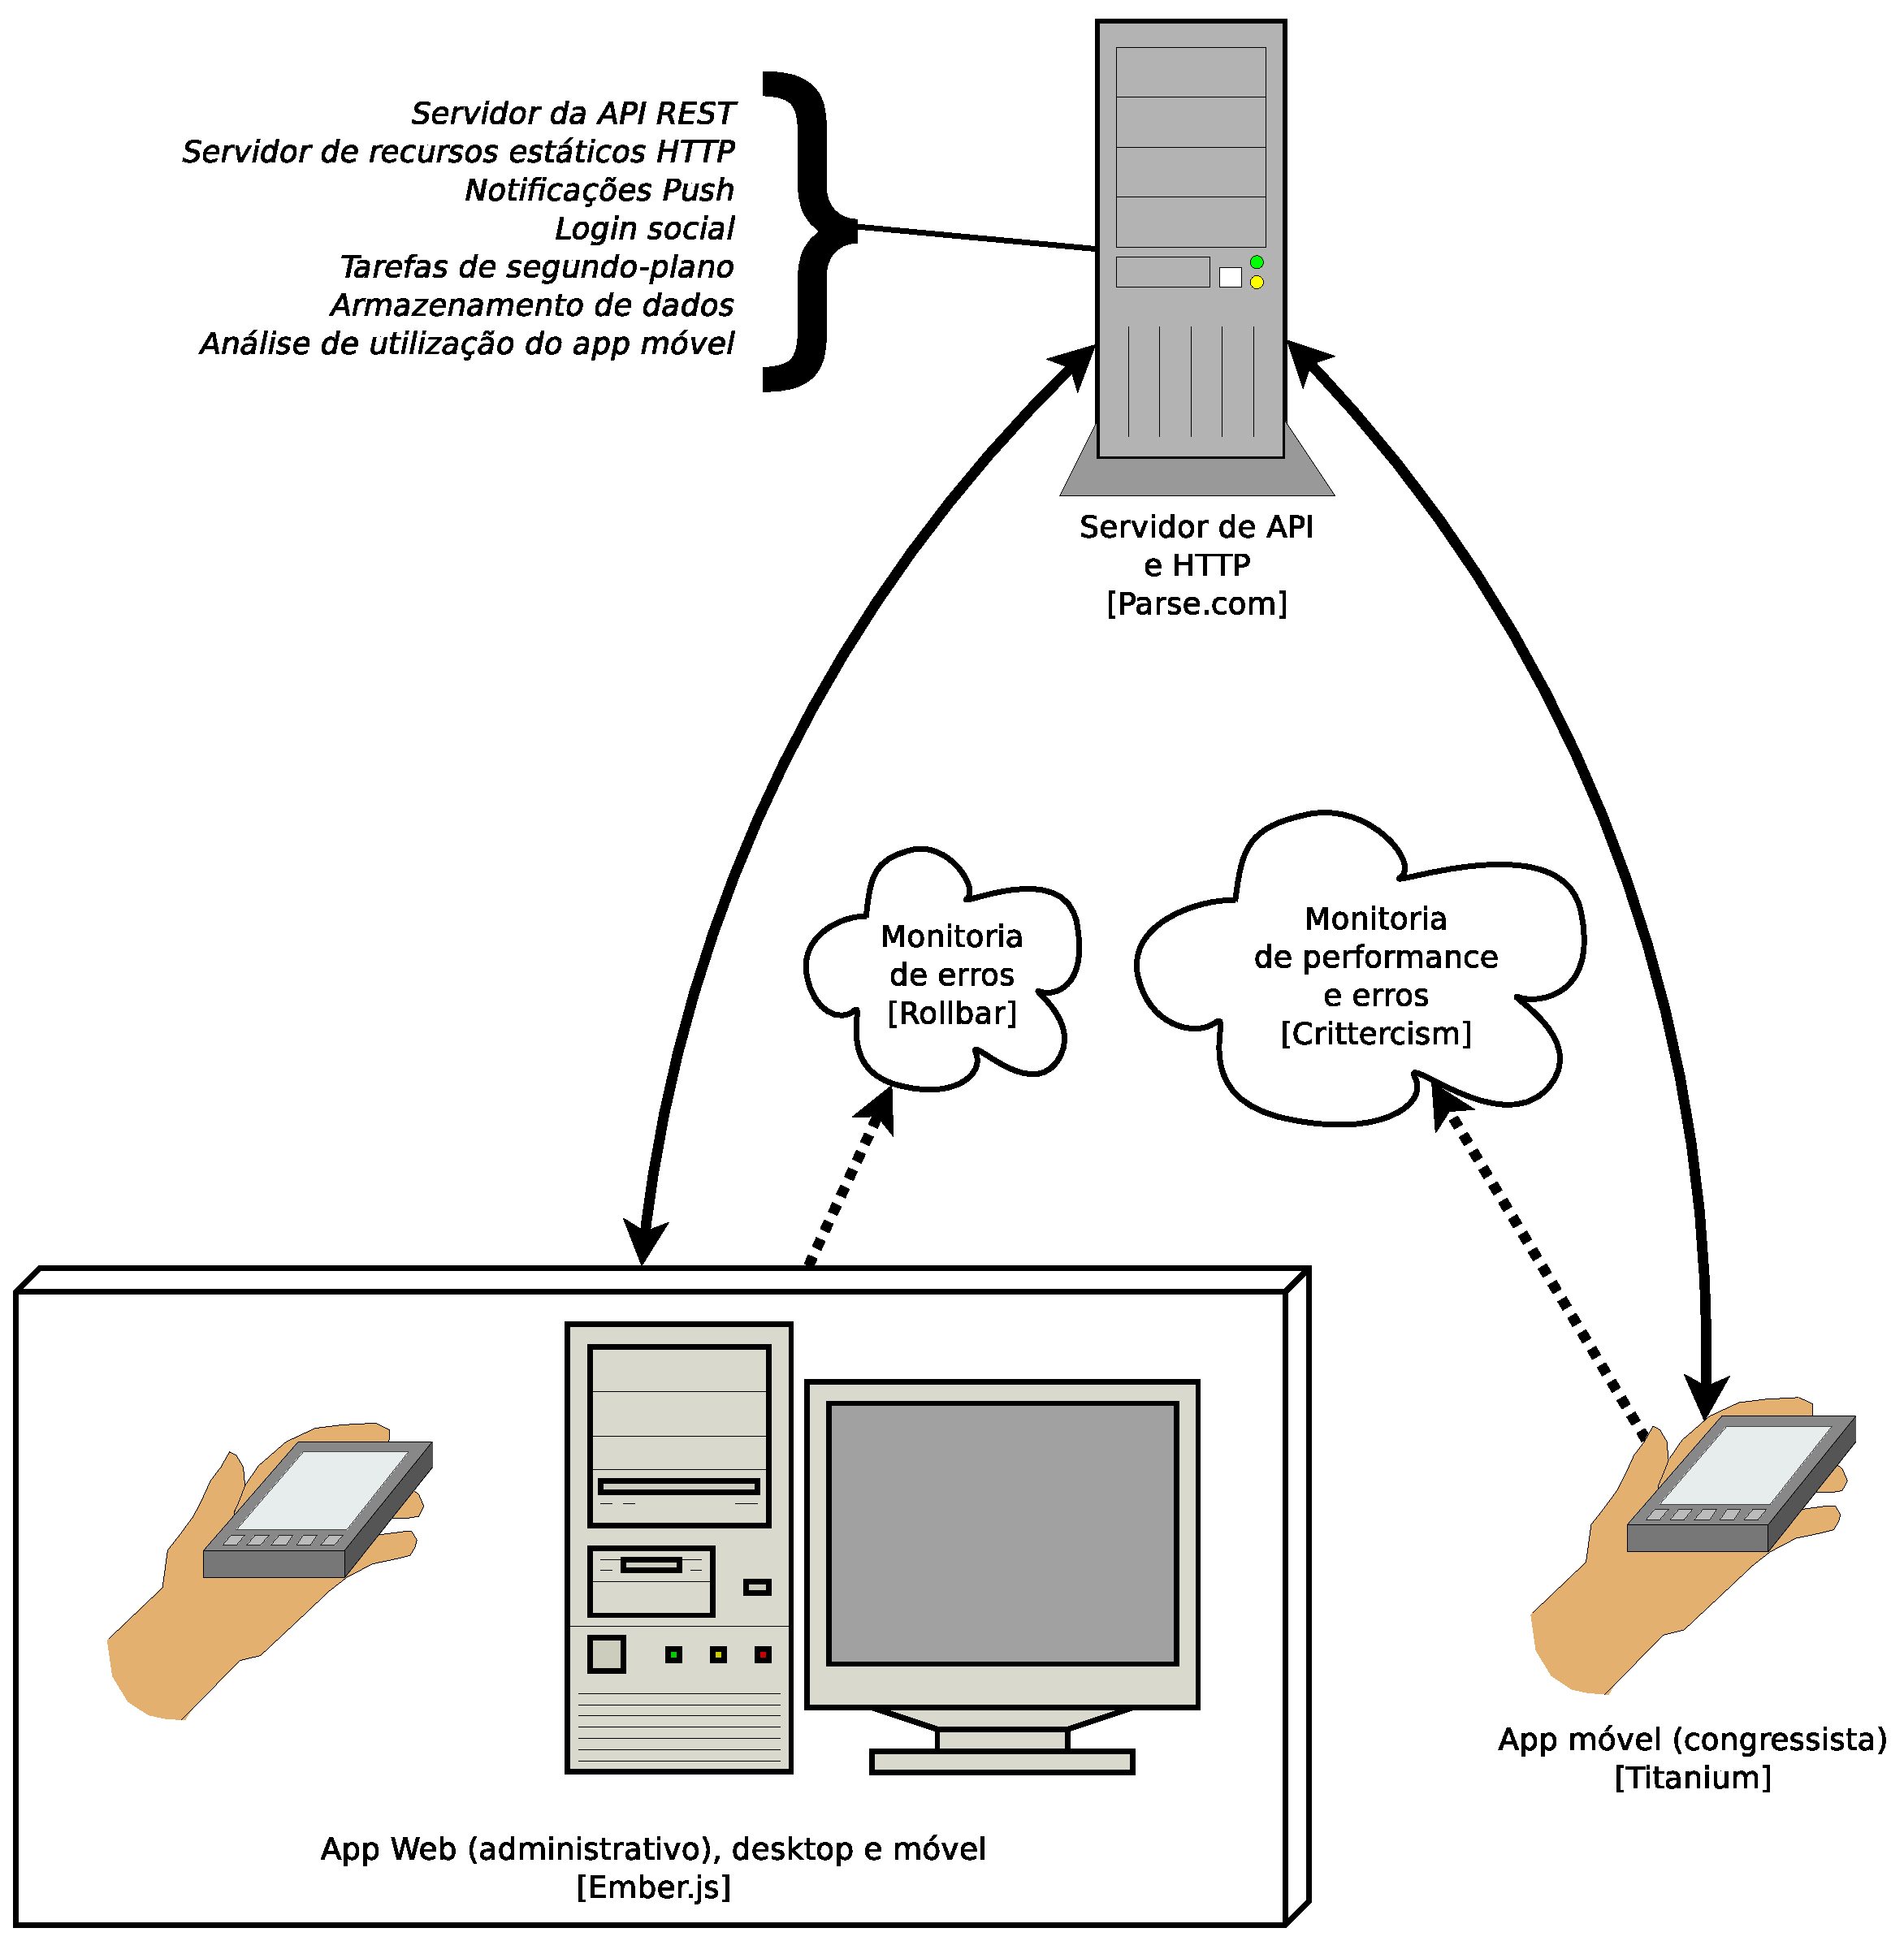
\includegraphics[width=0.8\linewidth]{diagramas/topologia-parse.eps}
	\caption{Diagrama de topologia simples, indicando o uso central dos serviços do Parse}
\end{figure}


%%%%%%%%%%%%%%%%%%%%%%%%%%%%%%%%%%%%%%%%%%%%%%%%%%%%%%%%%%%%%%%%%%%%%%%%%%%%%%%%%%%%%%%%%
\printbibliography

\end{document}